\section{Experimentos de qualidade}
\label{sec:experimentos-qualidade}
A heurística desenvolvida foi aplicada a alguns gráficos clássicos da
literatura, com o objetivo de avaliar o quão próximo da CMV a
cobertura de vértices produzida fica.

Para cada exemplo, serão apresentados o grafo, junto com a
CMV do mesmo. Além disso, serão apresentados três números:
\begin{description}
    \item[$n$] O número de vértices do grafo.
    \item[$k$] O número de vértices da CMV.
    \item[$k'$] O número de vértices da cobertura de vértices
    encontrada pela heurística.
\end{description}

As Figuras~\ref{fig:eq1}, \ref{fig:eq2}, \ref{fig:eq3} e~\ref{fig:eq4}
apresentam os grafos e seus respectivos resultados.

\begin{figure}[htb!]
\centering
\subfigure[Tetraedro\cite{cite:example-plato}, $n=4$, $k=3$, $k'=3$]{
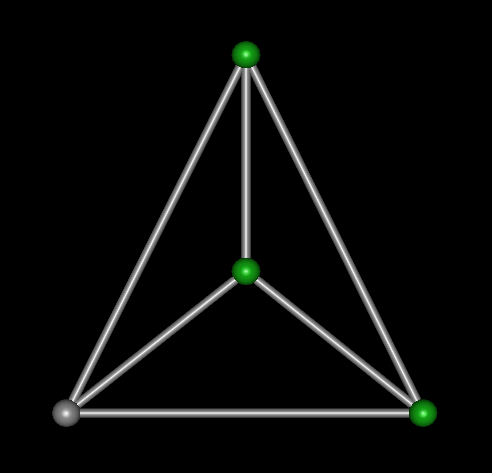
\includegraphics[width=0.4\textwidth]{img/tetraedro.png}
\label{fig:example-tetraedro}
}
\subfigure[Grafo bipartido de Kuratowski
    $K_{3,3}$~\cite{cite:example-kuratowski}, $n=6$, $k=3$, $k'=3$] {
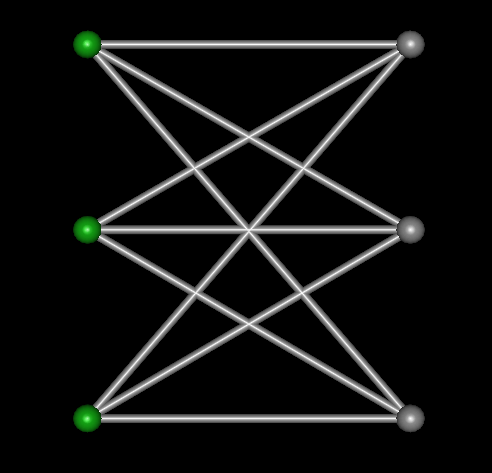
\includegraphics[width=0.4\textwidth]{img/kuratowski.png}
\label{fig:example-kuratowski}
}
\subfigure[Octaedro~\cite{cite:example-plato}, $n=6$, $k=4$, $k'=4$] {
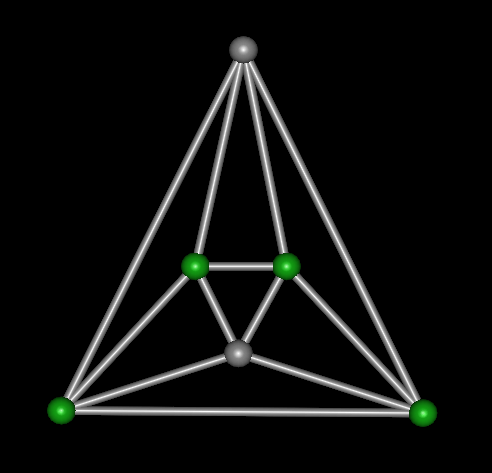
\includegraphics[width=0.4\textwidth]{img/octaedro.png}
\label{fig:example-octaedro}
}
\subfigure[Grafo de Bondy-Murphy $G_1$~\cite{cite:example-bondy},
    $n=7$, $k=4$, $k'=4$] {
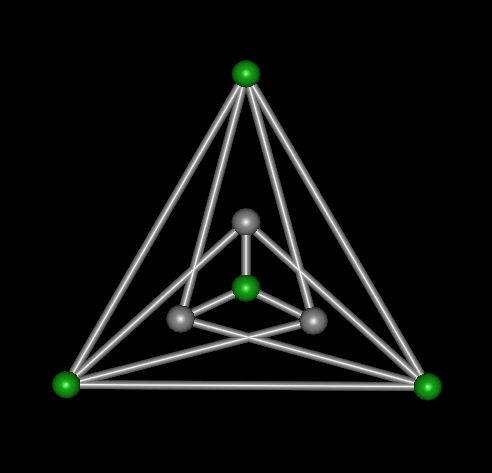
\includegraphics[width=0.4\textwidth]{img/bondymurphyg1.png}
\label{fig:example-bondymurphyg1}
}
\subfigure[Grafo roda $W_8$~\cite{cite:example-bondy}, $n=8$, $k=5$,
    $k'=5$] {
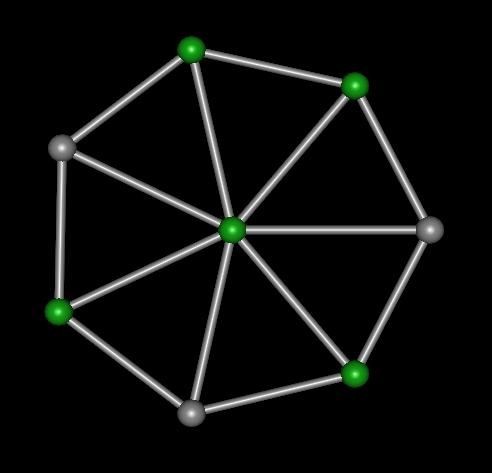
\includegraphics[width=0.4\textwidth]{img/wheel.png}
\label{fig:example-wheel}
}
\subfigure[Grafo cubo~\cite{cite:example-plato}, $n=8$, $k=4$, $k'=4$]
{
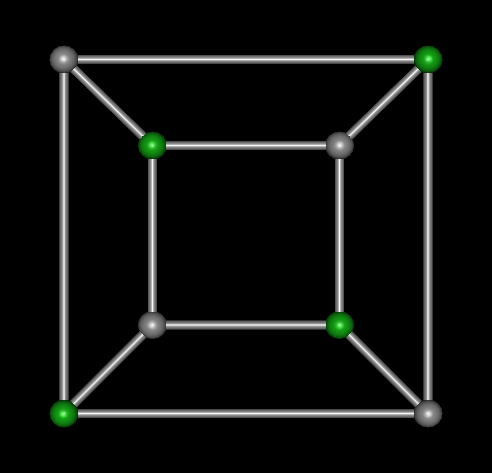
\includegraphics[width=0.4\textwidth]{img/cube.png}
\label{fig:example-cube}
}
\caption{Experimentos de qualidade}
\label{fig:eq1}
\end{figure}


\begin{figure}[htb!]
\centering
\subfigure[Grafo de Petersen~\cite{cite:example-petersen}, $n=10$,
    $k=6$, $k'=6$] {
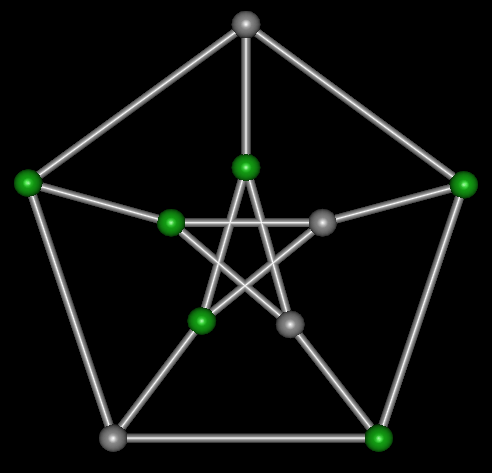
\includegraphics[width=0.4\textwidth]{img/petersen.png}
\label{fig:example-petersen}
}
\subfigure[Grafo de Bondy-Murphy $G_2$~\cite{cite:example-bondy},
    $n=11$, $k=7$,$k'=7$]{
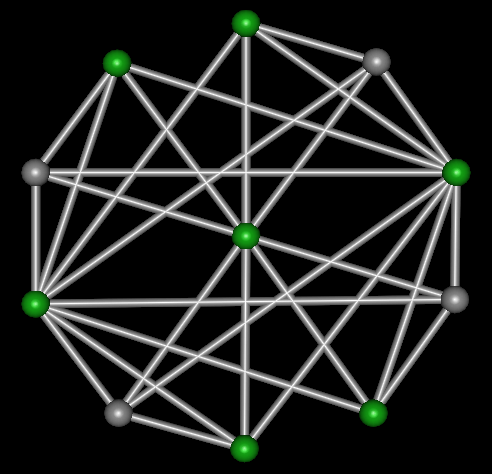
\includegraphics[width=0.4\textwidth]{img/bondymurphyg2.png}
\label{fig:example-bondymurphyg2}
}
\subfigure[Grafo de Grötzsch~\cite{cite:example-grotzsch}, $n=11$,
    $k=6$, $k'=6$]{
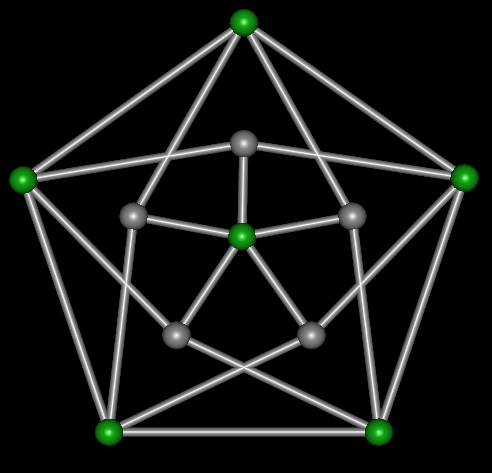
\includegraphics[width=0.4\textwidth]{img/grotzsch.png}
\label{fig:example-grotzsch}
}
\subfigure[Grafo de Herschel~\cite{cite:example-herschel}, $n=11$,
    $k=5$, $k'=5$] {
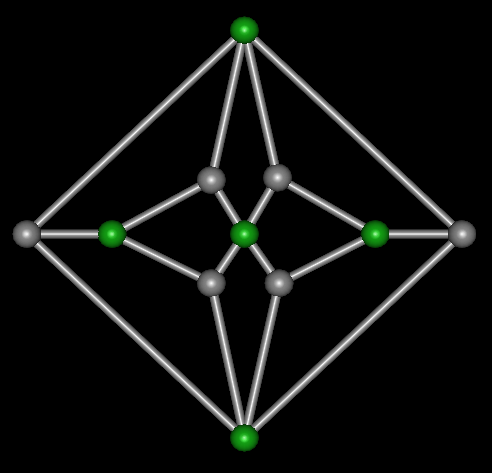
\includegraphics[width=0.4\textwidth]{img/herschel.png}
\label{fig:example-herschel}
}
\subfigure[Icosaedro~\cite{cite:example-plato}, $n=12$, $k=9$, $k'=9$]
{
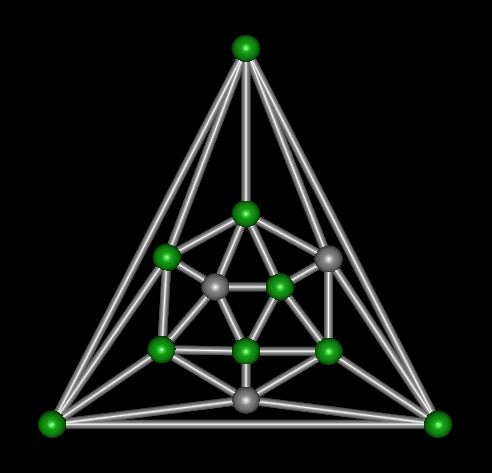
\includegraphics[width=0.4\textwidth]{img/icosaedro.png}
\label{fig:example-icosaedro}
}
\subfigure[Grafo de Bondy-Murphy $G_3$~\cite{cite:example-bondy},
    $n=14$, $k=7$, $k'=8$]{
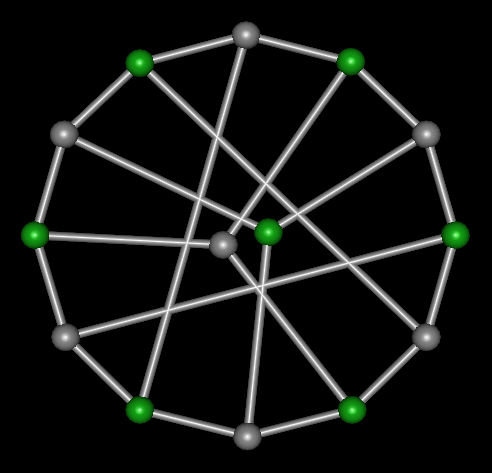
\includegraphics[width=0.4\textwidth]{img/bondymurphyg3.png}
\label{fig:example-bondymurphyg3}
}
\caption{Experimentos de qualidade}
\label{fig:eq2}
\end{figure}

\begin{figure}[htb!]
\centering
\subfigure[Grafo de Bondy-Murphy $G_4$~\cite{cite:example-bondy},
    $n=16$, $k=7$, $k'=7$]{
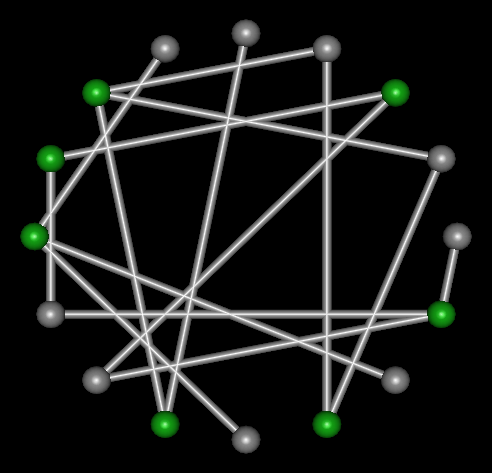
\includegraphics[width=0.4\textwidth]{img/bondymurphyg4.png}
\label{fig:example-bondymurphyg4}
}
\subfigure[Grafo de Ramsey $R(4,4)$~\cite{cite:example-ramsey},
    $n=17$, $k=14$, $k'=14$] {
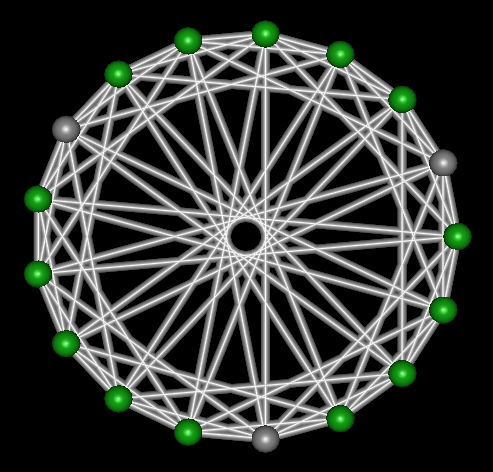
\includegraphics[width=0.4\textwidth]{img/ramsey.png}
\label{fig:example-ramsey}
}
\subfigure[Grafo de Folkman~\cite{cite:example-folkman}, $n=20$,
    $k=10$, $k'=10$]{
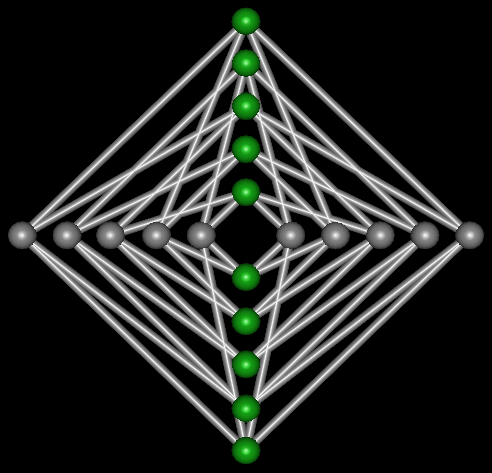
\includegraphics[width=0.4\textwidth]{img/folkman.png}
\label{fig:example-folkman}
}
\subfigure[Dodecaedro~\cite{cite:example-plato}, $n=20$, $k=12$,
    $k'=12$]{
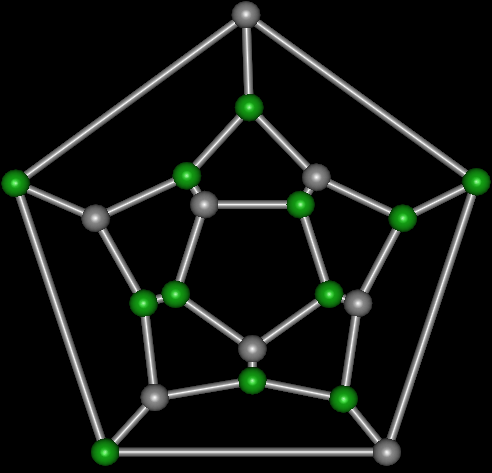
\includegraphics[width=0.4\textwidth]{img/dodecaedro.png}
\label{fig:example-dodecaedro}
}
\subfigure[Grafo de Tutte-Coxeter~\cite{cite:example-tutte}, $n=30$,
    $k=15$, $k'=15$]{
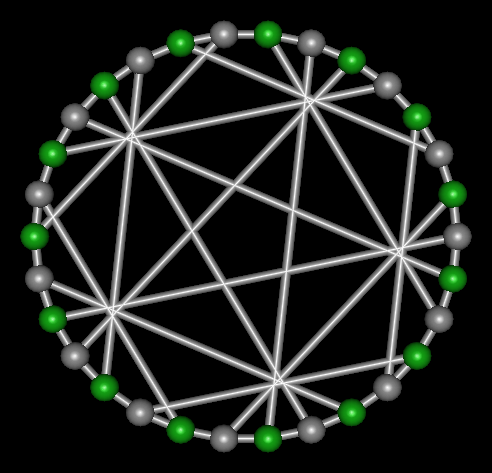
\includegraphics[width=0.4\textwidth]{img/tutte.png}
\label{fig:example-tutte}
}
\subfigure[Grafo de Thomassen~\cite{cite:example-thomassen}, $n=34$,
    $k=20$, $k'=20$]{
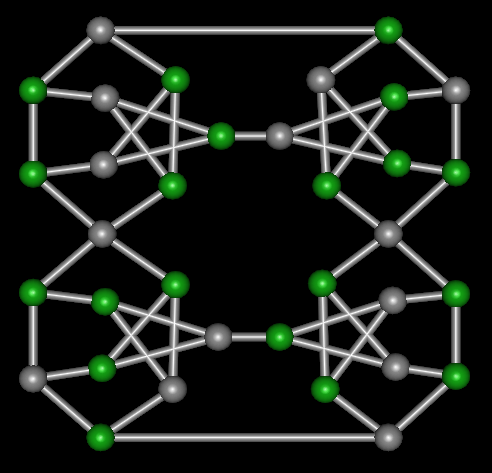
\includegraphics[width=0.4\textwidth]{img/thomassen.png}
\label{fig:example-thomassen}
}
\caption{Experimentos de qualidade}
\label{fig:eq3}
\end{figure}
\clearpage

\begin{figure}[htb!]
\centering
\subfigure[Grafo de Berge~\cite{cite:example-berge}, $n=60$, $k=40$,
    $k'=40$]{
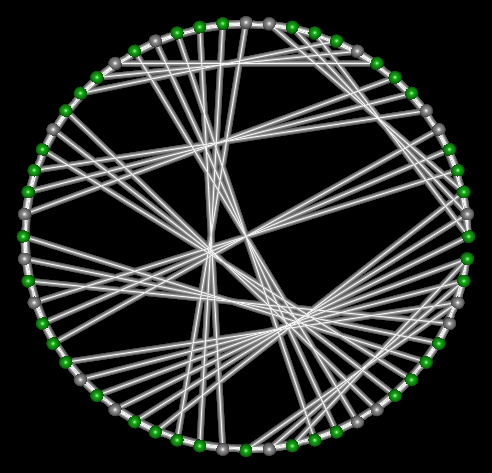
\includegraphics[width=0.4\textwidth]{img/berge.png}
\label{fig:example-berge}
}
\subfigure[Grafo de Witzel~\cite{cite:example-witzel}, $n=450$,
    $k=420$, $k'=429$]{
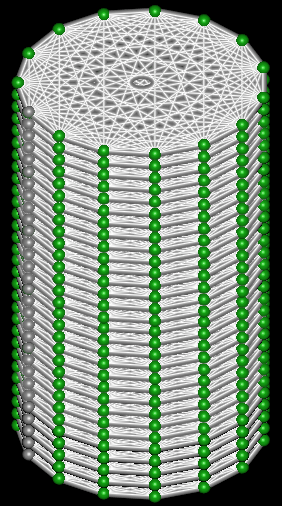
\includegraphics[width=0.4\textwidth]{img/witzel.png}
\label{fig:example-witzel}
}
\caption{Experimentos de qualidade}
\label{fig:eq4}
\end{figure}


\subsection{Análise}
Para quase todos os casos testados, com apenas duas exceções, a
heurística produziu uma resposta ótima para o grafo de entrada. E
mesmo nos dois grafos excepcionais (o grafo $G_3$ de Bondy-Murphy e o
grafo de Witzel) a resposta gerada ficou muito próxima do ótimo.

Claramente, as respostas geradas por esta heurística são
suficientemente boas.
